\documentclass[acmtog]{techreportacmart}

\usepackage{booktabs} % For formal tables


\usepackage[ruled]{algorithm2e} % For algorithms
\renewcommand{\algorithmcfname}{ALGORITHM}
\SetAlFnt{\small}
\SetAlCapFnt{\small}
\SetAlCapNameFnt{\small}
\SetAlCapHSkip{0pt}
\IncMargin{-\parindent}

% Copyright
\setcopyright{none}

\settopmatter{printacmref=false, printccs=false, printfolios=true}
\citestyle{acmauthoryear}
\setcitestyle{square}

% Document starts
\begin{document}
% Title portion
\title{Report: Deep Learning Methods for Reynolds-Averaged Navier-Stokes Simulations of
Airfoil Flows \\ Master-Seminar - Deep Learning in Physics} 
\author{Julian Hohenadel}
\affiliation{%
  \institution{Technical University of Munich}
}

\renewcommand\shortauthors{Hohenadel}

\begin{abstract}
This report aims to critically assess a deep learning approach to infer Reynolds-Averaged Navier-Stokes 
solutions. Following the thoughts of \cite{Thuerey20} a fully convolutional U-Net architecture is used 
to classify the performance on deriving pressure and velocity fields and their distributions. With an 
evaluation of different hyper parameter regarding network and training data size, the best models yield 
a mean error relative to pressure and velocity channels of less than 3\% on a test set containing 90 
samples. \cite{Thuerey20} states that due to this generic approach other PDE boundary value problems 
on Cartesian grids can also be tackled with this setup. In this report different adaptations of the 
network architecture are compared to each other with different data normalization in form of vector 
norms. Lastly the architecture is used to predict wave propagation on shallow water governed by the 
Saint-Venant equations.
\end{abstract}

%
% End generated code
%

\keywords{RANS, Reynolds-Averaged Navier-Stokes, CNN, U-Net, FCNN, PDE, CFD, Cartesian grid, 
pressure, velocity, airfoil, flow prediction, Eulerian field functions}


\thanks{This report is a part of the lecture, Master-Seminar - Deep Learning in
  Computer Graphics, Informatics 15, Technical University of Munich.}


\maketitle

\section{Introduction}
Since the last few years machine learning as well as deep learning in the form 
of neural networks enjoy great popularity. Their broad spectrum of application 
fields paired with the competitiveness of the researchers and fast available hardware (GPUs) 
allow the scientific community to squeeze out every bit of performance of their 
neural networks. \\
This hype also affects the computational fluid dynamics (CFD) field as \cite{viquerat2019}
shows with an exponential growth in published papers over the last 20 years.
Solving flow prediction problems traditionally is coupled with a deep understanding 
of physics and modeling these complex physical constrains. A neural network with a 
high enough capacity is capable to capture these high-dimensional, nonlinear constrains.
Neural networks are universal approximators \cite{Approximation} i.e.\ there is mostly a
trade-off regarding accuracy to the ground truth function (actual dynamics) and the 
number of parameter in the network. \\
\cite{Thuerey20} explains the first goal is to alleviate concerns regarding achievable accuracy
and analyzability of deep learning approaches by showing a relation between accuracy and
changes in the  hyper-parameter of a network.
As a second goal the paper provides a testing environment hosted on GitHub. 
Training data is also available which is a jump start for own experiments with computational fluid dynamics. Different training
dataset sizes and a flexible network capacity prevents long training time which can arise
from a potential hardware bottleneck. Using Google Colab different kinds of ReLu activation 
functions and their impact on the networks' accuracy are compared based on their mean errors 
regarding pressure, velocity and combined. Data preprocessing is one of the most important 
aspects to make the training fast and converge to good minima. For that reason different vector 
and pseudo norms are used to profit from dimensionless training data with different scaling. To prove 
that this generic setup as \cite{Thuerey20} claims is applicable to other partial differential equations 
(PDE) boundary value problems the network architecture is used to train on inferring the Saint-Venant 
equations, which \cite{Fotiadis2020} uses for the modeling of surface wave propagation.

% Figure
\begin{figure}[h]
  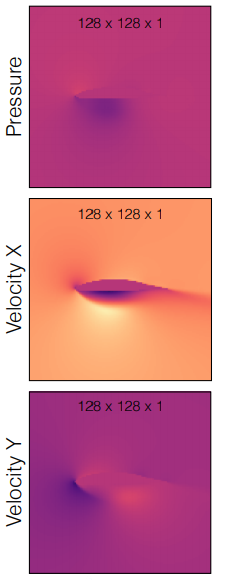
\includegraphics[width=.2\textwidth, height=.2\textheight]{figures/sampleTarget}
  %\vspace*{10mm}
  \caption{RANS infered pressure and velocity distributions around an airfoil.}
  \label{fig:zero}
\end{figure}

\section{Background}
Reynolds-averaged Navier-Stokes (RANS) equations are used for the modeling of turbulent incompressible flows \cite{Alfonsi}. \\
Due to inferring complexity as well as it's chaotic behaviour the Navier-Stokes equations are simplified by the RANS equations.
In the context of the paper RANS is used to infer 2D pressure and velocity distributions (see Figure ~\ref{fig:zero}) around airfoil shapes to predict
lift and drag coefficients.
The Navier-Stokes equation is a nonlinear partial differential equation which can be seen as Newtons's 2nd law of motion \cite{BISTAFA2018}:
% Numbered Equation
\begin{equation}
\label{eqn:01}
\frac{\partial{u}}{\partial{t}} + u \cdot \nabla u = g - \frac{1}{\rho} \nabla p + \nu \nabla^{2}u
\end{equation}
Where $u$ is the velocity vector, $g$ is the acceleration vector due to a body force, $p$ is pressure, 
$\nu$ is the kinematic viscosity and $\rho$ is the density. \cite{BISTAFA2018} rewrites the left side 
of the equation as the particles acceleration and the right side as the external forces that affect 
the particle per unit of mass which yields Newtons's 2nd law of motion.
The idea behind RANS is Reynolds decomposition which splits dependent model variables into a mean and fluctuating part \cite{Alfonsi}.
RANS averages over the time component, thus returning a single frame as infered solution.
The Reynolds number $Re$ is a dimensionless constant which is needed for the calculation of turbulence 
models. Depending on the magnitude of the Reynolds number the flow ranges from laminar to turbulent 
\cite{lissaman1983}. The angle of attack on an airfoil as well as the Reynolds number are important 
parameter for the creation of the physical model because they affect lift and drag coefficients \cite{lissaman1983}. 

\section{Method}
In the following the methodology used by \cite{Thuerey20} to infer the RANS solutions is summarized and 
extended by experiments evaluated for this report. For consistency reasons the structure is kept equal to the original paper.

\subsection{Data Generation}
The UIUC database \cite{airfoil} holds a variety of airfoil shapes, shown in Figure~\ref{fig:one}, which 
are used to generate training data. The provided data is only a 2D coordinate representation of the 
airfoil shape. To acquire the ground truth velocity and pressure maps the open source package OpenFOAM is 
used which contains solvers for CFD problems. The range of Reynolds numbers $[0.5, 5] \cdot 10^{6}$ used 
for generating the ground truth indicates turbulent airflow. Also, an angle of attack of $\pm 22.5$ degrees 
is used. RANS turbulence models distinguish between different classes \cite{Alfonsi}. In this case the 
one-equation model is used. The solutions are cropped to a resolution of $128x128$ pixels around the 
airfoil to speed up training while keeping the most relevant information. 
A test set is generated separately with unseen airfoil shapes.

% Figure
\begin{figure}[h]
  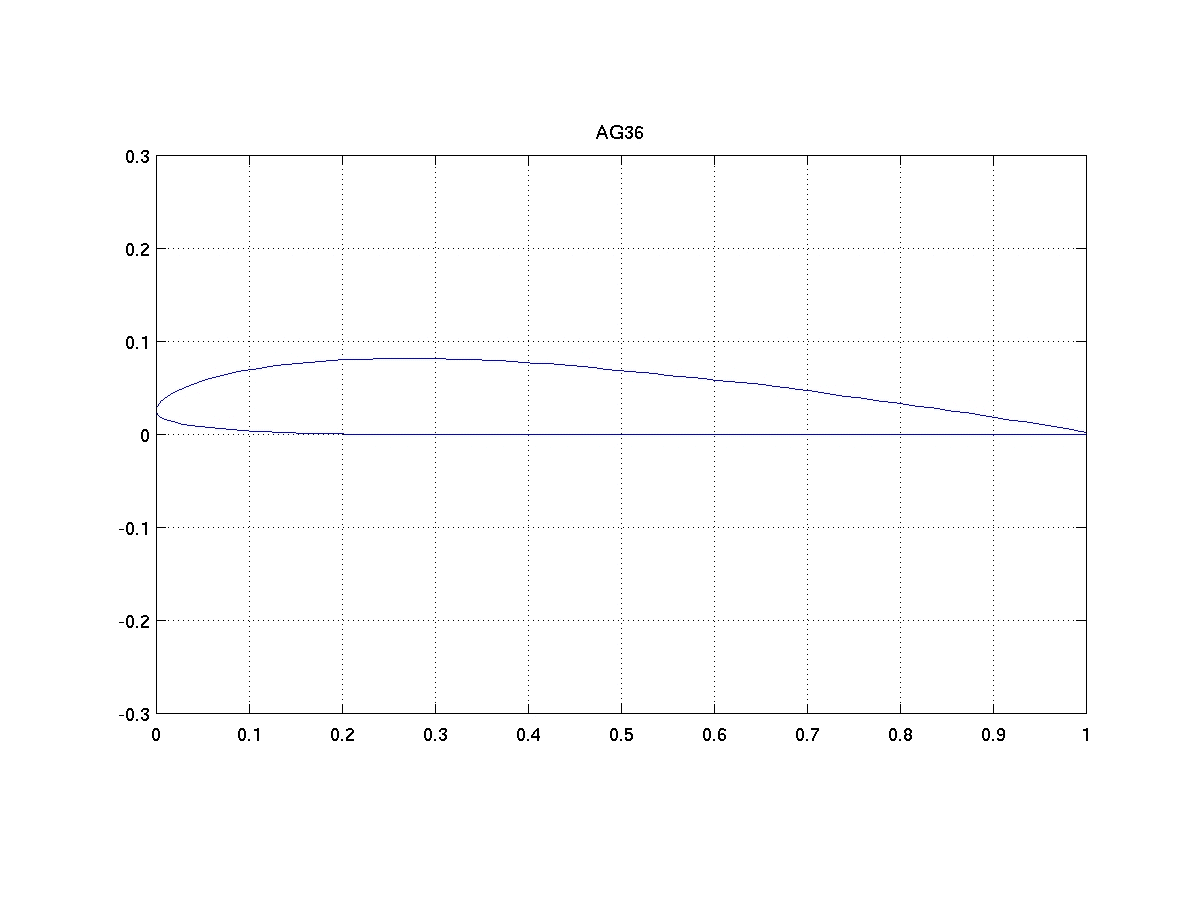
\includegraphics[width=.4\textwidth]{figures/uiuc_sample}
  \vspace*{-10mm}
  \caption{A sample airfoil shape in 2D.}
  \label{fig:one}
\end{figure}

\subsection{Pre-processing}
One training data sample consists of $3$ $128x128$ grids wrapped into a tensor. The channels are a bit 
mask representing the position and shape of the airfoil, $x$ and $y$ velocity. Inside the airfoil shape 
all elements contain $0$ in the velocity fields. The velocity maps are initialized with differently 
scaled freestream velocity vectors which have the corresponding Reynolds number for the sample encoded 
in them with respect to the magnitude of the elements. \\For the inferred solution of the neural network 
the shape stays the same as the input. Solutions are obtained from OpenFOAM as ground 
truth with channels split into pressure, $x$ and $y$ velocity.

\begin{equation}
\label{eqn:00}
	\frac{\textbf{v}^2}{2} + gz + \frac{\textbf{p}}{\rho} = constant
\end{equation}

The Bernoulli equation for incompressible laminar flow despite not beeing directly applicable for turbulent flow
motivates the first normalization step proposed in the paper. It shows a quadratic relation between velocity and
pressure. To make the data dimensionless the ground truth data is divided by the magnitude of the freestream 
velocity (default: L2 vector norm). The pressure channel is divided with the vector norm squared to remove the 
quadratic scaling as suggested by the Bernoulli equation.
In the context of physical units: In an incompressible model the density is constant so to make the 
pressure dimensionless it needs to be divided with the squared velocity. \\
% Table
\begin{table}
\caption{Norm comparision wrt. error, L2 default (in \%).}
\label{tab:one}
\begin{center}
\begin{tabular}{l|l|l|l|l}
  \toprule
  Norm   & pressure   &	velocity    & combined \\
  \bf L1	 & \bf 14.19	  & \bf 2.251		& \bf 2.646    \\
  L2	 & 14.76	  & 2.291		& 2.780	   \\
  L inf	 & 15.09	  & 2.348		& 2.865	   \\
  L 0.25 & 31.03	  & 3.106		& 3.272	   \\
  L 0.5  & 15.64	  & 2.448		& 2.705	   \\
  L 0.75 & 31.03	  & 3.106		& 3.272	   \\	
  \bottomrule
\end{tabular}
\end{center}
\bigskip\centering
\footnotesize L1 normalization achieves the best error rates (lower is better). \\
Trained on \cite{Thuerey20} U-Net implementation with $1.9 \cdot 10^{6}$ weights. \\
Seeds used for training: $0$, $2^{10}$, $2^{20}$, $2^{30}$
\end{table}%
Additionally, to norm based normalization the pressure channel is shifted into the origin 
by subtraction the pressure mean for each sample respectively. This is doable because the 
Navier-Stokes equations only use the pressure gradient $\nabla_p$ which allows for absolute pressure
values to be changed. By doing this the network does not have to waste resources on 
compensating for an off centered pressure map. Lastly \cite{Thuerey20} clamps each channel 
into an $[-1, 1]$ interval to ensure a maximum of numerical precision.


Table~\ref{tab:one} shows how different vector norms which are only used for normalization 
of the target data in the pre-processing step change the averaged error of neural networks 
which are all trained under the same conditions and capacity. 
$L1 \geq L2 \geq L_{inf}$ holds for every error channel. The other norms are quasi norms because they violate the required convexity 
but follow the same definition for a vector $x$:

% Numbered Equation
\begin{equation}
\label{eqn:02}
||x||_p := {\left( \sum_{i=0}^{n} |x_i|^p \right)}^{\frac{1}{p}}
\end{equation}

Surprisingly L$0.25$ and L$0.75$ normalization hold exactly the same results, although the absolute 
norm values on the same sample differ vastly. They also fail to infer target pressure values by 
around $2x$ when compared with the other norms. \\
Comparing the generated feature maps in the convolutional layers for the different normalizations
does not yield any precise information. The weight difference for each feature map does not seem to
follow any pattern besides increasing up to the bottleneck and then decreasing along the decoder. \\
Batch normalization is used to reduce internal covariance shift \cite{ioffe2015}. 
$\gamma$ and $\beta$ are two learnable parameters to influence variance and mean of the 
input data to improve training. Because \cite{Thuerey20} works with shuffled datasets 
it is not possible to directly compare the learned weights. The $\gamma$ and $\beta$ 
per layer mean differences between L1 and L2 normalization are in a range of $[10^{-3}, 10^{-2}]$. \\ 
It is not apparent why and how the weight changes affect the accuracy. Most likely the error 
improvement is far from being significant enough for a network with in this case close to 
$2 \cdot 10^{6}$ parameter. With bigger filter kernel sizes (e.g. VGG nets) in the convolutional 
layers the detected structures would be more comparable, while a maximal size of 4x4 pixels is limiting a visual comparison.

\subsection{Neural Network Architecture}
\cite{Thuerey20} use a modified version of the U-Net architecture proposed by \cite{ronneberger2015}. 
The U-Net architecture consists of two parts. The left side of the ``U`` functions as an encoder. 
It captures the context of the image. While width and height of the image get smaller the depth 
of the channels increases. The right side acts as a decoder. It upsamples the feature maps to 
recover spatial locations. The behavior of the image size and depth is contrary to the encoder 
part. Every block is implemented similarly: activation function (leaky ReLu in encoder, ReLu in 
decoder), convolution layer, batch normalization and finally dropout for regularization \cite{Thuerey20}. 
Without the help of skip connections information captured in the initial layers of the U-Net 
which is needed for reconstruction in the decoding part may get lost.\\ 
Activations control the flow of the gradients through the network which is essential for proper learning.
Rectified Linear Units (ReLu) and variants of ReLu are nowadays the standard choice as an activation function. 
ReLu does not saturate and yield large and consistent gradients. Both are important for fast convergence. 
The problem with ReLu is that it can ``die`` (e.g. the output is 0) which lowers the capacity of the 
network by deactivating neurons.
Leaky ReLu does have the same benefits as regular ReLu but does not suffer from the ``dying out`` problem. 
For this reason the same network architecture is trained with the activation setup \cite{Thuerey20} 
used as well as all activations set to vanilla ReLu and PReLu respectively. 
PReLu makes use of a learnable parameter which sets the negative slope through 
backpropagation while leaky ReLu has a fixed hard coded parameter for that reason ($0.2$ is used 
by \cite{Thuerey20}). 
Regular ReLu for both encoder and decoder is not a beneficial choice as information which is lost to 
the ``dead`` ReLu in the encoder can only be partially (with skip connections) or not at all be recovered 
and forwarded to the decoder. This shows in higher error rates especially for the pressure distribution.

\begin{table}[h]
\caption{Activation function comparision wrt. error after 160k iterations (in \%).}
\label{tab:two}
\begin{center}
\begin{tabular}{l|l|l|l|l}
  \toprule
  Activation   & pressure   &	velocity    & combined \\
  Std	 & 14.76	  & 2.29		& 2.78   \\
  \bf PReLu	 & \bf 14.69	  & \bf 2.21		& \bf 2.67	   \\
  ReLu   & 39.39	  & 2.97		& 3.17	  \\
  \bottomrule
\end{tabular}
\end{center}
\bigskip\centering
\footnotesize The PReLu activation function achieves  
the best error rates (lower is better). \\
Seed used for training: $0$
\end{table}%

Table~\ref{tab:two} shows that the standard setup could not achieve a better result while PReLu 
is able to slightly reduce the error by $0.1\%$. These results were obtained with a single seed and therefore 
may not be that conclusive but rather indicate a trend. PReLu activations on the encoder part have 
a mean parameter value close to the $0.2$ proposed by \cite{Thuerey20}. PReLu is also able to train 
one parameter for each input channel adding even more flexibility with the cost of additional weights. 

% Figure
\begin{figure}[h]
  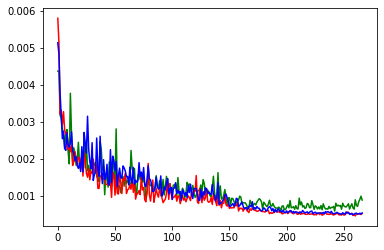
\includegraphics[width=.4\textwidth]{figures/val_loss}
  %\vspace*{-10mm}
	\caption{Validation loss comparison of Std (blue), PReLu (red), ReLu (green). \\
	Seed used for training: $0$}
  \label{fig:val}
\end{figure}

Figure ~\ref{fig:val} gives a good visual summary of the results.
The PReLu and standard setup both converge which explains their small error difference while the model
trained with only ReLu activations even starts to diverge.

\subsection{Supervised Training}
The training setup used by \cite{Thuerey20} consists of an $L_1$ loss, learning rate decay and the 
use of the Adam optimizer \cite{kingma2014adam} with default PyTorch settings except $\beta_1$ 
(set to $0.5$). Lowering $\beta_1$ slows down acceleration but can be 
useful if you overshoot good local minima. 
While the $30.9m$ model suffers from its huge capacity in form of overfitting 
small data sets it achieves a combined relative error of $2.6\%$ using the $12.8k$ sample training 
dataset. The $1.9m$ and $7.7m$ model also show close results wrt. the highest capacity model.\\
\cite{Thuerey20} explore generalization with an additional dataset in which the airfoil shapes 
were sheared by $\pm15\%$. This reduced the error to $2.32\%$ when training 
with a $51k$ mixed dataset ($30.9m$ model). 
\cite{Thuerey20} achieves a speed up of ca. $1000x$ when using an NVidia GTX 1080 
GPU for inference of the neural networks compared to OpenFOAM.

\section{Transfer}
To show another use case for the models created by \cite{Thuerey20} they will be used to infer 
the propagation of surface waves governed by the Saint-Venant equations as they are related with 
the Navier-Stokes equations which is examined in \cite{Fotiadis2020}. For this experiment the 
U-Net architecture will be the same except the input channels of the first layer which now contain 
the last $n$ time steps. The same is applied to the output of the last layer to predict the next 
$m$ time steps. As a testing environment the GitHub repository provided by \cite{Fotiadis2020} is 
used. To be consistent with \cite{Fotiadis2020} U-Net architecture and to make the results comparable 
$n=5$ and $m=20$ without dropout is used in this setup. Due to Google Colab hardware and runtime 
restrictions both models were only trained for 50 epochs and both neural nets have a capacity 
between $[7.7 \cdot 10^6, 7.8 \cdot 10^6]$.\\
omparing Figure~\ref{fig:T2} to Figure~\ref{fig:T1} both RMSE are almost similar up to 35 
time-steps ahead and after 80 time-steps the gap is still relatively small. 
\cite{Fotiadis2020} achieve with their U-Net a speed-up of 241x compared with numerical 
simulations. 

% Transfer 1
\begin{figure}[h]
  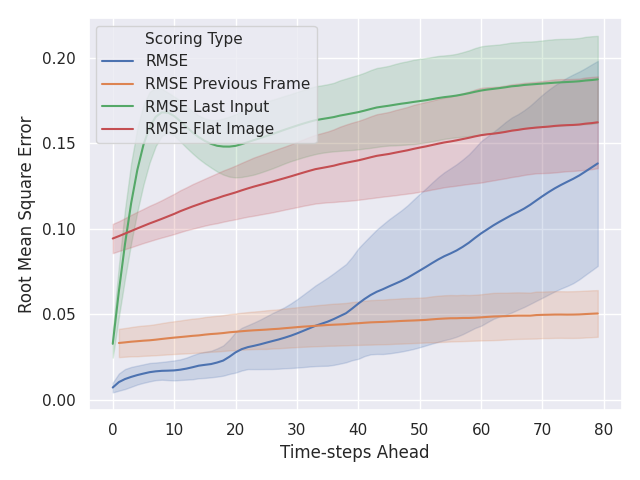
\includegraphics[width=.35\textwidth]{figures/transfer/DFP_Test_RMSE_Quality_start_15}
  \caption{RMSE error on test set with \cite{Thuerey20} architecture.}
  \label{fig:T1}
\end{figure}

% Transfer 2
\begin{figure}[h]
  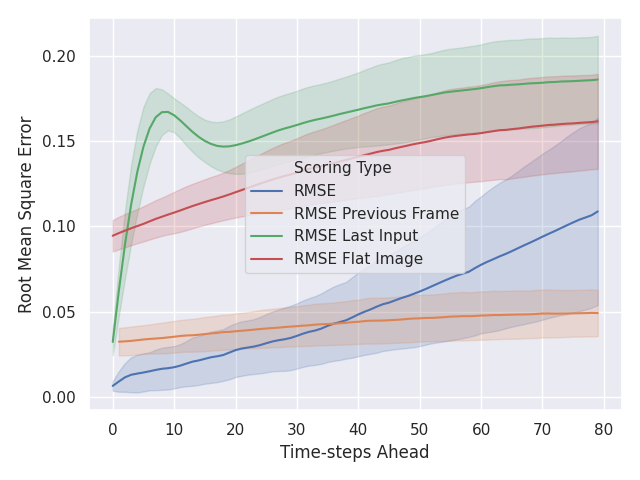
\includegraphics[width=.35\textwidth]{figures/transfer/Transfer_Test_RMSE_Quality_start_15}
  \caption{RMSE error on test set with \cite{Fotiadis2020} architecture.}
  \label{fig:T2}
\end{figure}

\section{Generalization}
Generalization performance is measured with an extrapolation and interpolation approach shown 
in Table ~\ref{tab:gen1} and ~\ref{tab:gen2} respectively. \\
The ground truth for the training data works with an angle of attack interval of $[-22.5, 22.5]$ degrees
for training as well as testing. Increasing the interval yields a lower relative error increase when compared
with an interval shift. While the ground truth interval is still a subset in the increased interval the 
shifted interval does not overlap which explains the drastic error increase.\\
The error increase in the interpolation setting is caused by the neural network 
not being able to infer pressure and velocity distributions on the opposite part of the airfoil wrt.
the angle of attack.


% Table
\begin{table}
	\caption{Error increase for different angle of attack intervals (test set) in \%.}
\label{tab:gen1}
\begin{center}
\begin{tabular}{l|l|l|l|l}
  \toprule
  Interval   		& pressure   &	velocity    & combined \\
  $[-45, 45]$	 	& 3.66	  & 5.14		& 6.07	   \\
  $[-90, 90]$	 	& 5.73	  & 19.20		& 18.23	   \\
  $[-67.5, -22.5]$ 	& 6.00	  & 13.84		& 15.11	   \\
  $[22.5, 67.5]$  	& 10.7	  & 23.25		& 22.99	   \\
  \bottomrule
\end{tabular}
\end{center}
\bigskip\centering
	\footnotesize Extrapolation of AoA intervals, ground truth: $[-22.5, 22.5]$ \\
\end{table}%

% Table
\begin{table}
\caption{Error increase for different angle of attack intervals in \%.}
\label{tab:gen2}
\begin{center}
\begin{tabular}{l|l|l|l|l}
  \toprule
  Interval   	& pressure   &	velocity    & combined \\
  $[-22.5, -10]$ 	& 4.64	  & 12.66		& 11.38	   \\
  $[10, 22.5]$	 	& 2.5	  & 10.13		& 9.37	   \\
  \bottomrule
\end{tabular}
\end{center}
\bigskip\centering
\footnotesize Interpolation of AoA intervals, ground truth interval splitted \\
	into train and test (shown) intervals, no intersections.  
\end{table}%

\section{Discussion}
\cite{Fotiadis2020} show that U-Nets can outperform LSTM's in accuracy as well as in speed 
up with a fraction of capacity (in time-series problems). Convolutions paired with an encoder 
decoder structure seem to catch regions of interest fast and reliable. Looking at the validation 
and mean error plots shown in \cite{Thuerey20} the accuracy does not suffer too much from models 
with a lot less capacity. Their natural regularization effect should make improvement possible 
even with a small mixed dataset which would again increase inference speed. It is not clear 
why problem specific solver should infer airfoil flows if the accuracy of neural networks 
can be improved even more. \cite{Thuerey20} show that the data pre-processing (i.e. reducing 
the space of solutions) is almost more important than the actual fine-tuning of the models. 
This research is important because it questions the use of solvers and shows the rapid progress 
wrt. accuracy of convolutional neural networks in CFD problems.

\section{Conclusion} 
\cite{Thuerey20} present an out-of-the-box well training derivative of the U-Net architecture 
proposed by \cite{ronneberger2015}. Despite being firstly designed for image segmentation it is 
applicable in a wide variety of research fields. This report compared different vector and pseudo 
norms for the pre-processing step and their influence on the training process. PReLu as an activation 
function is compared to classic ReLu and leaky ReLu. While hard coded activation parameter can provide 
good training results after hyper parameter tuning it can be worth testing activations that train 
themselves through backpropagation. For the cost of some additional weights given enough iterations 
it may be worth considering. The U-Net being applicable to other PDE problems leaves a lot of possible 
future work especially because convolutional neural networks are able to outperform LSTM's in time-series predictions.\\

\newpage
% Bibliography
\bibliographystyle{ACM-Reference-Format}
\bibliography{sample-bibliography}

\end{document}
